\question[20] A 50 gram firecracker is initially at rest when it explodes into three pieces which move away in different directions. Immediately after the explosion, the first piece, which has a mass of 16 grams, moves with a speed of 22 m/s at an angle of $\theta=60^\circ$ relative to the $x$ axis. The second piece (20 g) moves directly backward with a speed of 14 m/s. These two pieces are illustrated in the figure below.

\begin{center}
	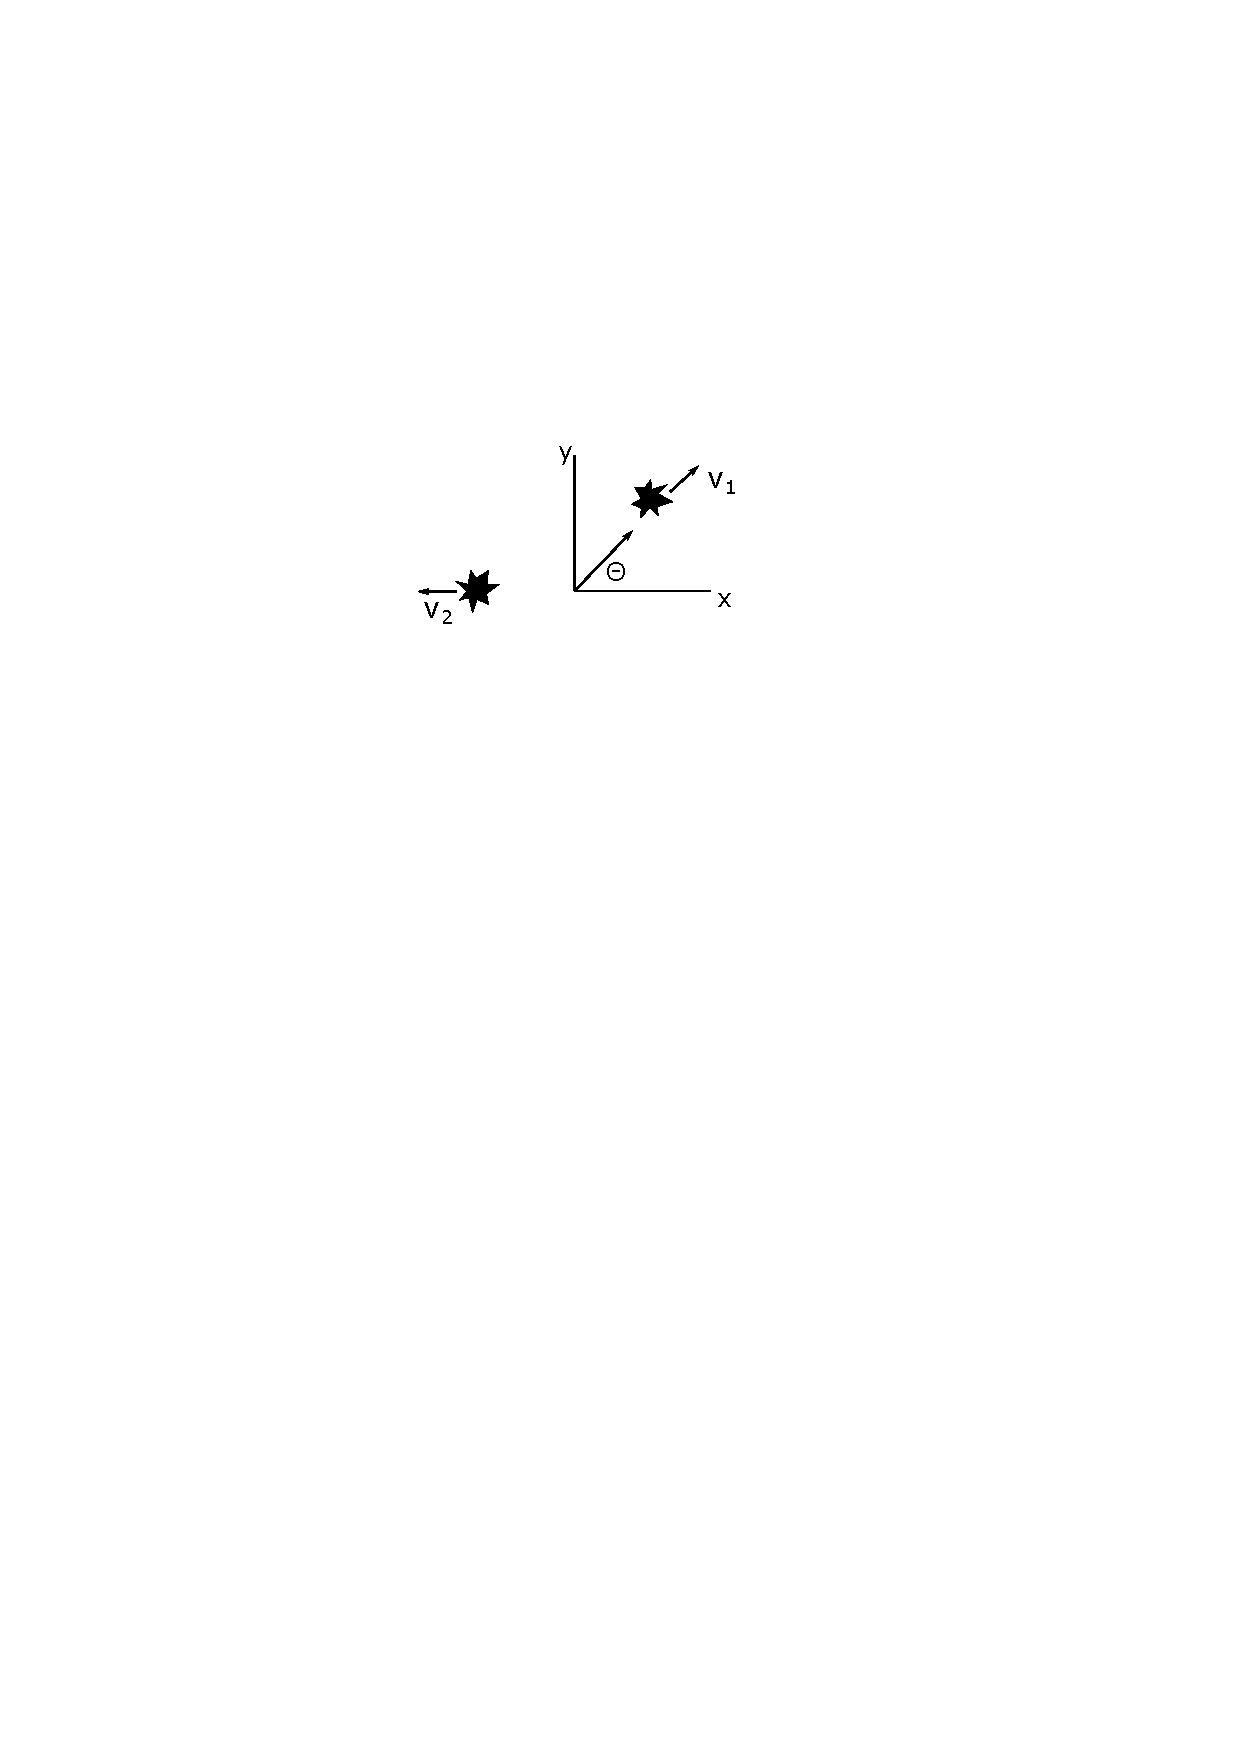
\includegraphics[width=5cm]{explosion.pdf}
\end{center}

\begin{parts}
	\part With what speed and in what direction does the third piece move after the explosion? (Express your direction as an angle relative to the $x$ axis)
	\vspace{8 cm}
	\part The three pieces went from being motionless initially to moving with great speed after the explosion. Was energy conserved in the explosion? Explain.
\end{parts}